\documentclass{assignment}
\usepackage{amsmath}
\usepackage{lipsum}
\usepackage{multicol}
\usepackage{fancyhdr}
\usepackage{graphicx}
\usepackage{blindtext}
\usepackage[dvipsnames]{xcolor}
\usepackage{enumitem}
\usepackage{cleveref}
\usepackage{color,soul}
\usepackage{amsfonts}
\newcommand{\indicator}[1]{\mathbf{1}_{\{#1\}}}
\def\code#1{\texttt{#1}}
\newtheorem{anm}{Anm}

\begin{document}


\assignmentTitle
{Lucas Frykman}{0210127650}
{SF1930}
{Liam Solus}
{assets/KTH_logga.png}
{Statistisk inlärning och dataanalys}
{Projekt}

% \section*{Introduktion}
% Vi betraktar den skateboard tävlingen.

\section{Uppvärmning}

\begin{figure}[!h]
    \caption{Histogram av betyg skalad mellan 0 och 1}
    \begin{center}
        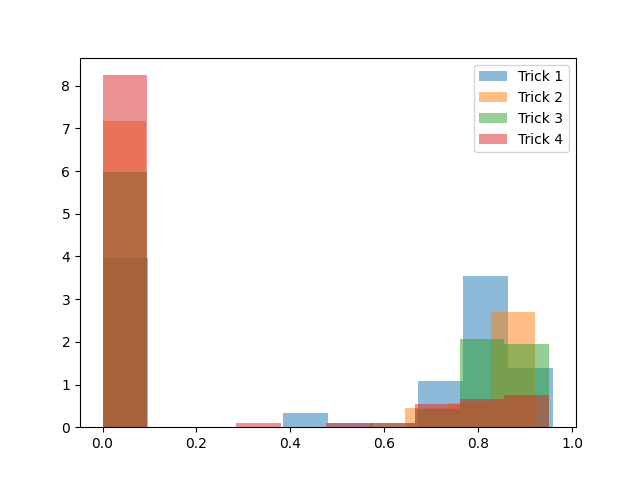
\includegraphics[width = 99mm]{assets/Figure_2.png} \label{Histogram 1}
    \end{center}
\end{figure}


Låt $B$ vara betyg för en ett skateboardåkare och trick. Vi vill skatta $P(B>0.6|B>0) = \frac{P(B>0|B>0.6)P(B>0.6)}{P(B>0)}=\frac{P(B>0.6)}{P(B>0)}$
som $\tilde{P}(B>0.6|B>0) = \frac{\sum_{i}^4\sum_{j}^{96}trick_{ij}\indicator{[0.6,1]}}{\sum_{i}^4\sum_{j}^{96}trick_{ij}\indicator{[0,1]}} \approx 0.96$
Det här stämmer med utseendet på \cref{Histogram 1}.

\begin{figure}[!h]
    \caption{Spridningsdiagram mellan run 1 och run 2}
    \begin{center}
        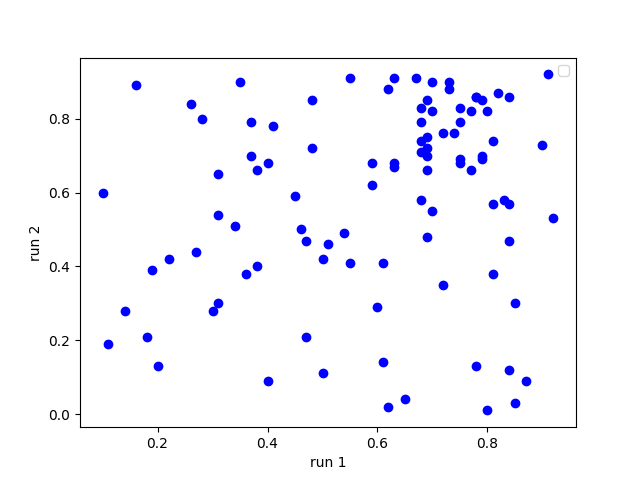
\includegraphics[width = 99mm]{assets/Figure_1.png}
    \end{center}
\end{figure}

\newpage
\section{En frekventistisk modell}
\begin{anm} \label{properties}
    Vår model för $X_i$ är följande 
    \\ $X_i = \left\{\begin{matrix}
        0 \text{ om } V_i=0
        \\ Z_i \text{ om } V_i=1
    \end{matrix}\right.$
    \\ där $V_i \sim \text{Ber}(\theta_i)$ och $Z_i\sim \text{Beta}(\alpha_i,\beta_i)$ det här är ekvivalent med att säga
    \\ $V_i = \indicator{x\neq0}(X_i)$ och $Z_i= X_i|(V_i=1)$ 
    \\ eftersom det här är bara en transformation av stokatiska variebler ger stickprov från $X_i$ oss ett stickprov för $Z_i$ och $V_i$
\end{anm}

\subsection*{(a) Skatta $\theta_{i}$}

Låt $x_{i[n]} = (x_{i1},x_{i2},...x_{in})^T$ vara vår stickprov från samtliga trick skateboardåkaren $i$ utförde.
\begin{align}
    L(\theta_{i},\alpha_{i},\beta_{i}|x_{i[n]}) = \prod_{j=1}^nf_{x_{i}}(x_{ij}) = \prod_{j}^n (1-\theta_i) \indicator{x=0} (x_{ij}) + \theta_if_{Z_i}(x_{ij})\indicator{x\neq0}(x_{ij})
    \\ \Longleftrightarrow \nonumber
    \\ L(\theta_{i},\alpha_{i},\beta_{i}|x_{i[n]}) = (1-\theta_i)^{n-m}\theta_i^{m}\prod_{j=1}^n\left(f_{Z_i}(x_{ij})\indicator{x\neq0}(x_{ij}) + \indicator{x=0}(x_{ij})\right) 
\end{align}
där $m=\sum_{j=1}^n \indicator{x\neq0}(x_{ij})$ alltså hur många gånger $x_{i}$ inte är noll (gånger tävlaren $i$ landade tricket).
Nu tar vi log likliehoodfunktionen.
\begin{align}
    \Longrightarrow \log(L) = (n-m)\log(1-\theta_i)+m\log(\theta_i)+ \sum_{j=1}^n \log \left(f_{Z_i}(x_{ij})\indicator{x\neq0}(x_{ij}) + \indicator{x=0}(x_{ij})\right) \label{loglike}
    \\ \Longleftrightarrow \partial_{\theta_i}\log(L) = \frac{m-n}{1-\theta_i} + \frac{m}{\theta_i} = 0 \label{blah}
    \\ \Longleftrightarrow \frac{m-n\theta_i}{\theta_i(1-\theta_i)} = 0 \Longleftrightarrow \hat{\theta_i} = \frac{m}{n} \label{MLE result}
\end{align}
MLE för bernoulli fördelningens $V_i$ parameter $\hat{\theta_i} = \text{argmax}_{\theta\in\Omega} L(\theta_i|v_{i[n]}) = \bar{v_i}$ skulle ge oss samma resultat. Eftersom vi kan transformera stickprovet $x_{i[n]}\rightarrow v_{i[n]}$ med \cref{properties} $v_i=\indicator{x\neq0}(x_i)$.
vilket betyder att $m=\sum_{j=1}^n v_i$ och därmed får \cref{MLE result} att sammanfalla med MLE av bernoulli fördelningen. 
\subsection*{(b) skatta $\alpha$ och $\beta_i$}
Observera att från \cref{loglike}  $\sum_{j=1}^n \log \left(f_{Z_i}(x_{ij})\indicator{x\neq0}(x_{ij}) + \indicator{x=0}(x_{ij})\right) = \sum_{j=1}^n \log \left(f_{Z_i}(x_{ij})\indicator{x\neq0}(x_{ij})\right)$ eftersom $\log(1)=0$.
Vi vet att 
\\ $\text{argmax}_{\alpha,\beta\in\Omega}\log(L)=\text{argmax}_{\alpha,\beta\in\Omega}\sum_{j=1}^n \log \left(f_{Z_i}(x_{ij})\indicator{x\neq0}(x_{ij})\right)$ vilket är ekvivalent med 
\\$\text{argmax}_{\alpha,\beta\in\Omega} \log(L(\alpha,\beta|z_{i[k]}))$ för att $z$ stickprovet innehåller alla trick som landade $z_{i[k]}=(z_{i1},\dots z_{ik})^T = \left\{x_{ij}\in x_{i[n]} : x_{ij}\neq 0\right\}$
\\ Vi ska alltså bara maximera log-likelihood av beta fördelningens paramtrerna givet data from $Z_i$

\begin{align*}
    \left\{\begin{matrix}
        \partial_{\alpha}\log(L(\alpha,\beta|z_{i[k]})) = \sum_{j=1}^k \partial_\alpha \log(f(z_{ij})) = 0
        \\ \\ \partial_{\beta}\log(L(\alpha,\beta|z_{i[k]})) = \sum_{j=1}^k \partial_\beta \log(f(z_{ij})) = 0
        \end{matrix}\right.
    \\ 
    \\ \text{:: } \partial_\alpha\log(f(z_{ij})) = \partial_\alpha\log \left( \frac{\Gamma(\alpha + \beta)}{\Gamma(\alpha) \cdot \Gamma(\beta)} \cdot z_{ij}^{\alpha-1} \cdot (1-z_{ij})^{\beta-1}\right) 
    \\  = \partial_\alpha \left(\log \Gamma(\alpha + \beta) - \log\Gamma(\alpha) - \log \Gamma(\beta) + (\alpha-1) \log z_{ij} + (\beta-1)\log (1-z_{ij}) \right)
    \\  = \partial_\alpha\log(f(z_{ij})) = \psi(\alpha+\beta) - \psi(\alpha) + \log z_{ij} \text{  där  } \psi = \Gamma ' / \Gamma 
    \\ \left(\text{Vi gör liknande för } \partial_\beta \log f(z_{ij}) \right)
    \\ \Rightarrow 
    \left\{\begin{matrix}
        \partial_{\alpha}\log L= k\psi(\alpha+\beta)-k\psi(\alpha) + \sum_{j=1}^k\log(z_{ij}) = 0
        \\ \\ \partial_{\beta}\log L= k\psi(\alpha+\beta)-k\psi(\beta) + \sum_{j=1}^k\log(1-z_{ij})) = 0
        \end{matrix}\right.
\end{align*}


\section{En bayesiansk modell}
\section{En bayesiansk modell med en hierarki}
\section{Diskussion}

% \section{Kod}
% \lstinputlisting[language=Matlab,caption=foo]{assets/tmp.m} 
\end{document}
